\documentclass[10pt,a4paper]{article}
\usepackage[utf8]{inputenc}
\usepackage[T1]{fontenc}
\usepackage[french]{babel}
\usepackage{geometry}
\usepackage{graphicx}
\usepackage{tabularx}
\usepackage{booktabs}
\usepackage{array}
\usepackage{enumitem}
\usepackage{xcolor}
\usepackage{hyperref}
\usepackage{titlesec}

\geometry{margin=1.7cm}
\graphicspath{{../}{doc/}}
\hypersetup{colorlinks=true,linkcolor=black,urlcolor=blue,pdftitle={NutriMatch - Architecture et STRIDE}}

\setlength{\parindent}{0pt}
\setlength{\parskip}{0.42em}
\linespread{1.06}
\setlength{\emergencystretch}{2em}
\renewcommand{\arraystretch}{1.24}
\setlist[itemize]{leftmargin=*,itemsep=0.18em,topsep=0.2em}
\setlist[enumerate]{leftmargin=*,itemsep=0.18em,topsep=0.2em}
\titlespacing*{\section}{0pt}{0.85em}{0.35em}
\titlespacing*{\subsection}{0pt}{0.65em}{0.25em}
\newcolumntype{Y}{>{\raggedright\arraybackslash}X}
\newcolumntype{L}[1]{>{\raggedright\arraybackslash}p{#1}}

\begin{document}

\begin{titlepage}
  \centering
  \vspace*{1.7cm}
  {\Huge\bfseries NutriMatch\par}
  \vspace{0.45cm}
  {\Large Architecture applicative, DFD, STRIDE et mesures de securite\par}
  \vspace{0.8cm}
  {\large Application de recommandation nutritionnelle securisee\par}

  \vspace{1.6cm}
  \begin{tabularx}{0.86\textwidth}{@{}L{3.1cm}Y@{}}
    \toprule
    \textbf{Etudiant 1} & \textbf{[Nom Prenom etudiant 1]} -- Specialite: \textbf{[Specialite etudiant 1]} \\
    \textbf{Etudiant 2} & \textbf{[Nom Prenom etudiant 2]} -- Specialite: \textbf{[Specialite etudiant 2]} \\
    \bottomrule
  \end{tabularx}

  \vfill
  {\large Backend Go, Frontend Next.js, PostgreSQL/pgvector, Redis\par}
  \vspace{0.25cm}
  {\large Catalogue local et IA explicative controlee\par}
\end{titlepage}

\section{Objectif et perimetre}
NutriMatch genere des recommandations de repas personnalisees selon le profil nutritionnel de l'utilisateur. Le systeme prend en compte les aliments aimes, les aliments moins apprecies, les allergies, les intolerances, les ingredients exclus, les maladies fermees et les medicaments declares.

La priorite du projet est la securite. Une recette dangereuse ne doit jamais etre proposee si elle viole une contrainte dure. Le backend reste donc l'autorite absolue: l'IA n'ajoute pas de recette externe, ne contourne pas les regles medicales et ne peut valider qu'une recette deja filtree par le moteur deterministe.

\section{Architecture et stack technique}
\begin{tabularx}{\textwidth}{@{}L{3.2cm}Y@{}}
\toprule
\textbf{Composant} & \textbf{Role dans l'application} \\
\midrule
Frontend Next.js / React & Landing page, inscription, connexion, onboarding, resultats, choix de recette, profil et securite compte. Les pages protegees redirigent vers la connexion si la session est absente. \\
Backend Go / Gin & API REST, clean architecture, validation stricte, authentification, MFA, profil nutritionnel, moteur de recommandation, audit et orchestration IA. \\
PostgreSQL + pgvector & Persistance par schemas: identite, sante, catalogue local, recommandations, traces, audit et similarite vectorielle deterministe. \\
Redis & Support partage pour rate limiting, session/cache applicatif et reduction de charge. \\
Google AI optionnel & Validation et explication de recettes deja considerees sures par le backend. Les erreurs IA sont classees et exposees sans fuite de secret. \\
Docker Compose & Stack locale complete: base pgvector, Redis, migrations Goose, API compilee et frontend compile. \\
\bottomrule
\end{tabularx}

Le backend suit une clean architecture: handlers HTTP, middlewares, services metier, repositories et modeles. Les controles de securite ne sont pas delegues au frontend: chaque payload est revalide cote serveur.

\section{Fonctionnement metier}
\begin{enumerate}
  \item L'utilisateur cree un compte, obtient une session puis complete son profil nutritionnel.
  \item Le backend normalise les entrees, refuse les champs inconnus et calcule le profil nutritionnel utile.
  \item Le catalogue local complet est charge depuis PostgreSQL; aucune API recette externe n'est dans le chemin critique.
  \item Les hard constraints bloquent sans negociation: allergies, allergies croisees, ingredients exclus, maladies, medicaments et regles nutritionnelles.
  \item Les soft constraints influencent seulement le score: aliments aimes, aliments moins apprecies, objectif, similarite et diversite.
  \item Le backend tire jusqu'a vingt recettes dans le pool deja sur, puis demande a l'IA de confirmer et expliquer ces recettes.
  \item Si l'IA rejette une recette, le backend la retire pour la fenetre courante, tire une autre recette deja sure et relance la validation.
  \item Le set quotidien est conserve vingt-quatre heures. Une recette choisie est affichee seule et exclue des futures suggestions pendant sept jours.
\end{enumerate}

\section{DFD logique et flux de donnees}
\begin{center}
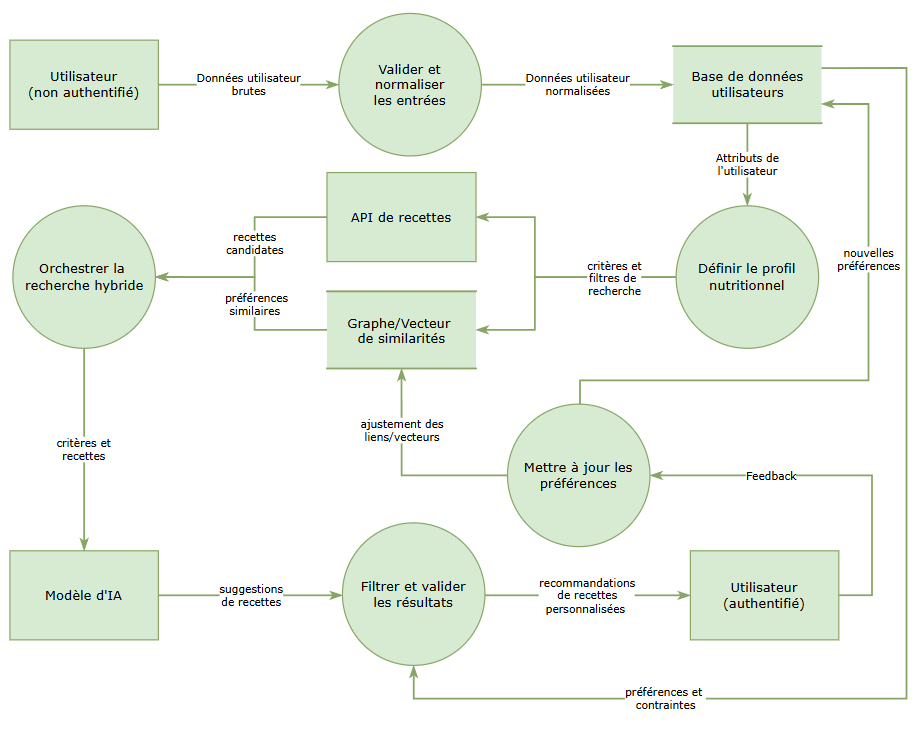
\includegraphics[width=0.91\textwidth]{dfd_v3.png}
\end{center}

\begin{itemize}
  \item \textbf{Utilisateur vers frontend}: saisie du compte, profil, preferences et contraintes.
  \item \textbf{Frontend vers API}: requetes authentifiees, token CSRF pour mutations et access token court en memoire.
  \item \textbf{API vers PostgreSQL}: ecriture cloisonnee dans les schemas identite, sante, catalogue, recommandation et securite.
  \item \textbf{API vers Redis}: rate limit, session/cache et coordination legere.
  \item \textbf{API vers IA}: seulement des faits minimises sur des recettes deja filtrees; aucune donnee brute de sante inutile.
  \item \textbf{API vers frontend}: recettes validees, raisons metier, et explications IA seulement si la validation IA a reussi.
\end{itemize}

\section{Modeles, donnees et cloisonnement}
\begin{tabularx}{\textwidth}{@{}L{3.2cm}Y@{}}
\toprule
\textbf{Schema} & \textbf{Contenu principal} \\
\midrule
\texttt{identity} & Utilisateurs, credentials, sessions, refresh tokens, MFA TOTP, passkeys WebAuthn et challenges. \\
\texttt{health} & Profil, mensurations utiles, preferences, contraintes et donnees sensibles chiffrees. \\
\texttt{catalog} & Recettes locales, ingredients, alias, allergies, allergies croisees, maladies et compatibilites medicales. \\
\texttt{recommendation} & Sets quotidiens, repas du set, choix utilisateur, rejets IA, details de preparation et traces. \\
\texttt{security} & Audit trail, hash-chain, evenements de securite, rate buckets et retention. \\
\bottomrule
\end{tabularx}

Le role applicatif PostgreSQL est separe du super-utilisateur local. Les donnees sensibles sont chiffrees au niveau applicatif avant persistance lorsque necessaire, et les index aveugles permettent certaines comparaisons sans exposer la valeur brute.

\newpage
\section{STRIDE par composant}
\subsection{1. Frontend Next.js et navigateur}
\begin{tabularx}{\textwidth}{@{}L{1.6cm}L{4.2cm}Y@{}}
\toprule
\textbf{S} & Session volee ou page protegee ouverte sans session. & Guard via proxy Next.js, redirection vers \texttt{/login}, refresh cookie HttpOnly et access token uniquement en memoire. \\
\textbf{T} & Manipulation du formulaire ou valeurs canoniques forcees. & Le frontend n'est pas fiable: validation finale cote API, taxonomie serveur et refus des champs inconnus. \\
\textbf{R} & Action utilisateur non tracable. & Les mutations sensibles generent des evenements d'audit cote backend avec request ID. \\
\textbf{I} & XSS, fuite DOM, stockage local de donnees sante. & CSP avec nonce, pas de stockage persistant du profil sante dans le navigateur, cookies HttpOnly. \\
\textbf{D} & Abus de formulaires auth/profil. & Rate limiting cote API, body limit et validations par etape. \\
\textbf{E} & Navigation directe vers pages protegees. & Middleware/proxy de session et verification serveur sur chaque endpoint protege. \\
\bottomrule
\end{tabularx}

\subsection{2. API Go, routes et middlewares}
\begin{tabularx}{\textwidth}{@{}L{1.6cm}L{4.2cm}Y@{}}
\toprule
\textbf{S} & Requete anonyme se faisant passer pour un utilisateur. & JWT signe, expiration courte, session liee au token et verification de session active. \\
\textbf{T} & JSON malforme ou injection de champs non prevus. & Binding JSON strict, DTO limites, normalisation serveur et validation go-playground/validator. \\
\textbf{R} & Absence de preuve apres incident. & Audit trail append-only, correlation request/session/user et resultat de l'action. \\
\textbf{I} & Fuite par erreur API ou logs. & Reponses d'erreur standardisees, secrets jamais renvoyes, details fournisseur IA non exposes. \\
\textbf{D} & Payloads volumineux ou flood endpoints. & Limite de body, rate limit Redis/PostgreSQL et timeouts externes. \\
\textbf{E} & BOLA/IDOR sur \texttt{profileId} ou recommandations. & Controle proprietaire de ressource dans les services et routes authentifiees. \\
\bottomrule
\end{tabularx}

\subsection{3. Authentification, sessions, CSRF et MFA}
\begin{tabularx}{\textwidth}{@{}L{1.6cm}L{4.2cm}Y@{}}
\toprule
\textbf{S} & Vol de credentials ou refresh token. & Mot de passe Argon2id, refresh token en cookie HttpOnly, hash du refresh avec pepper, rotation refresh et revocation logout. \\
\textbf{T} & CSRF sur refresh/logout/profil. & Token CSRF lie a la session, double submit cookie, header obligatoire, Origin/Referer de confiance. \\
\textbf{R} & Deni de changement mot de passe ou MFA. & Audit des changements password, MFA, passkeys, sessions et echecs de connexion. \\
\textbf{I} & Lecture du refresh token par JavaScript. & Cookie HttpOnly, SameSite configurable, Secure obligatoire en production. \\
\textbf{D} & Bruteforce login ou MFA. & Rate limiter, suivi des echecs auth, blocage temporaire et TTL de challenges MFA. \\
\textbf{E} & Acces fort sans second facteur configure. & MFA optionnel mais complet: TOTP, passkeys WebAuthn, preference MFA et challenge uniquement si active. \\
\bottomrule
\end{tabularx}

\subsection{4. Profil sante et moteur nutritionnel}
\begin{tabularx}{\textwidth}{@{}L{1.6cm}L{4.2cm}Y@{}}
\toprule
\textbf{S} & Lecture du profil d'un autre utilisateur. & User ID issu du token, ownership check et endpoints profil authentifies. \\
\textbf{T} & Contrainte medicale modifiee ou incoherente. & Taxonomie fermee pour maladies, ingredients canoniques, normalisation, validation et recalcul serveur. \\
\textbf{R} & L'utilisateur nie une contrainte renseignee. & Audit des modifications de profil, contraintes et recalculs nutritionnels. \\
\textbf{I} & Donnees sante exposees au repos. & Chiffrement AES-256-GCM cible, index aveugles, minimisation des champs et prompt IA reduit. \\
\textbf{D} & Profil trop verbeux ou trop complexe. & Budgets de texte, limites de listes et rejet des payloads excessifs. \\
\textbf{E} & Soft constraint transformee en bypass sante. & Hierarchie stricte: hard constraints avant soft scoring, similarite et IA. \\
\bottomrule
\end{tabularx}

\subsection{5. Catalogue local, recommandations et IA}
\begin{tabularx}{\textwidth}{@{}L{1.6cm}L{4.2cm}Y@{}}
\toprule
\textbf{S} & Source recette externe non controlee. & Catalogue local primaire en base; suppression de l'API recette externe du chemin critique. \\
\textbf{T} & IA modifie l'ordre, ajoute une recette ou ignore une allergie. & Contrat JSON strict, IDs autorises uniquement, champs interdits refuses, revalidation backend apres IA. \\
\textbf{R} & Impossible d'expliquer une recommandation. & Traces de set quotidien, raisons metier, rejets IA, selection mode et decision summary. \\
\textbf{I} & Prompt contenant donnees sensibles inutiles. & Payload IA minimise: recettes deja sures, ingredients, contraintes abstraites et pas d'identifiant direct. \\
\textbf{D} & Recalcul couteux a chaque affichage. & Cache quotidien vingt-quatre heures, choix cache et exclusion sept jours. \\
\textbf{E} & Recette dangereuse acceptee par hasard ou similarite. & Pare-feu deterministe: allergies, allergies croisees, exclusions, maladies, medicaments et compatibilite medicale. \\
\bottomrule
\end{tabularx}

\subsection{6. PostgreSQL, Redis et Docker}
\begin{tabularx}{\textwidth}{@{}L{1.6cm}L{4.2cm}Y@{}}
\toprule
\textbf{S} & Connexion BDD avec droits trop larges. & Role applicatif separe du compte admin local et variables d'environnement dediees. \\
\textbf{T} & Alteration de traces ou donnees catalogue. & Migrations versionnees, audit hash-chain, repository pattern et transactions controlees. \\
\textbf{R} & Perte d'historique apres incident. & Audit immutable logique, retention configuree et traces securite separees. \\
\textbf{I} & Exposition de ports ou secrets Docker. & Ports lies a \texttt{127.0.0.1}, reseaux internes Compose, secrets via env, pas de secrets en dur applicatifs. \\
\textbf{D} & Saturation DB/cache. & Healthchecks, Redis pour rate limit/cache, indexes, pgvector et timeouts. \\
\textbf{E} & Contournement par service interne. & Services separes, dependances Compose explicites, API demarre apres migrations et DB healthy. \\
\bottomrule
\end{tabularx}

\newpage
\section{Mesures de securite implementees}
\begin{tabularx}{\textwidth}{@{}L{3.8cm}Y@{}}
\toprule
\textbf{Domaine} & \textbf{Mesures concretes} \\
\midrule
Identite locale & Inscription/connexion, hachage Argon2id, politique longueur mot de passe, changement de mot de passe avec ancien mot de passe, confirmation et revocation des sessions pertinentes. \\
Refresh et sessions & Access token court en memoire, refresh token HttpOnly, hash refresh en base avec pepper, rotation au refresh, logout avec revocation, idle TTL et expiration. \\
MFA & TOTP complet, passkeys WebAuthn, challenge MFA conditionnel, preference MFA, desactivation controlee et audit des evenements MFA. \\
CSRF et origine & CSRF lie a la session, cookie CSRF lisible pour header, verification cookie/header, controle Origin/Referer et origines de confiance configurables. \\
CORS et cookies & CORS restreint aux origines autorisees, credentials controles, SameSite configurable, \texttt{Secure} obligatoire en production et chemins cookies dedies. \\
Frontend security & CSP avec nonce, \texttt{frame-ancestors 'none'}, protections headers, pas de profil sante stocke cote navigateur, access token non persistant. \\
Validation entrees & JSON strict, refus des champs inconnus, limites de taille body, budgets texte, normalisation email/texte/ingredients et taxonomie fermee. \\
Controle d'acces & Ownership checks sur profil, nutrition, recommandations, trace et choix de repas; routes sensibles authentifiees. \\
Chiffrement repos & AES-256-GCM pour donnees sensibles ciblees, chiffrement des secrets MFA et index aveugles avec cle separee. \\
Audit trail & Evenements auth, CSRF, MFA, profil, recommandations, choix, rejets, erreurs IA; hash-chain, append-only logique et request/session correlation. \\
Retention & Parametres de retention pour audit, echecs auth, rate buckets, sessions et traces de recommandation. \\
Rate limiting & Backend compatible Redis ou PostgreSQL, buckets dedies, limitation auth et routes HTTP pour reduire brute force et DoS. \\
Catalogue local & Import nettoye, trim/dropna/deduplication, ingredients canoniques, allergies, allergies croisees et compatibilite maladie-recette. \\
Pare-feu nutritionnel & Blocage deterministe des allergies, intolerances, allergies croisees, ingredients exclus, maladies, medicaments et plafonds nutritionnels critiques. \\
Soft constraints & Likes, dislikes, objectif et similarite ne font que ponderer; elles ne peuvent jamais annuler une contrainte dure. \\
IA controlee & Pool deja safe, contrat JSON strict, refus des IDs inconnus, refus des champs interdits, pas de score IA, pas de mock explanation, erreurs IA classees. \\
Cache recommandations & Set quotidien vingt-quatre heures, exclusions du set precedent si possible, exclusion sept jours apres choix et cache du detail IA choisi. \\
Docker & Images versionnees, PostgreSQL pgvector, Redis, migrations Goose automatiques, ports locaux standards, reseaux internes et healthchecks. \\
\bottomrule
\end{tabularx}

\section{Paradigmes de securite}
\textbf{Zero Trust.} Le navigateur, le reseau, les donnees entrantes et l'IA sont consideres non fiables. Toutes les decisions critiques sont reprises cote backend.

\textbf{Defense in Depth.} Le meme flux est protege par plusieurs couches: CSP, CORS, CSRF, JWT, session active, validation, chiffrement, audit, rate limit et controle metier.

\textbf{Fail-Safe Defaults.} En cas d'erreur medicale, de sortie IA invalide ou de doute sur une recette, la recette est rejetee ou l'explication IA est absente. Aucune contrainte dure n'est relachee.

\textbf{Least Privilege.} Separation des schemas, role applicatif dedie, prompt IA minimal, ports Docker limites localement et services separes.

\textbf{Privacy by Design.} Les donnees inutiles sont retirees, les donnees sensibles sont chiffrees, les prompts sont minimises et les logs evitent les secrets.

\section{Limites assumees et conclusion}
La version locale fonctionne en HTTP pour faciliter le developpement. Pour une production reelle, il faut imposer HTTPS, activer \texttt{COOKIE\_SECURE=true}, utiliser des secrets forts, restreindre les origines HTTPS, proteger les logs, externaliser la supervision et appliquer TLS vers toute base distante.

NutriMatch est donc structure comme une application de recommandation nutritionnelle securisee: catalogue local, backend autoritaire, hard constraints non negociables, IA controlee et auditabilite complete des decisions sensibles.

\end{document}
